\documentclass[a4paper,12pt]{article}
\usepackage[utf8]{inputenc}
\usepackage[margin=25mm]{geometry}
\usepackage{setspace}
\usepackage{amsmath}
\usepackage{courier}
\usepackage{enumitem}
\usepackage{hyperref}
\usepackage[style=authoryear, natbib,backend=bibtex]{biblatex}
\addbibresource{bibliography.bib}
\usepackage{graphicx}


\setlength{\parskip}{1\baselineskip plus 1pt minus 1pt}
\setlength{\parindent}{0pt}

\begin{document}

% Title Page
\begin{titlepage}
    \centering
    \vspace*{1in}
    \Huge
    \textbf{Detailed Project Proposal (DPP)}

    \vspace{0.5in}
    \LARGE
    Leveraging Deep Features for ORB-SLAM3 (DXSLAM-ORB3)

    \vspace{1.5in}
    \large
    Student Name: Adwaith Kallungal Vrundavanan \\
    Student ID: 22061390\\
    MSc in AI and Robotics \\
    Supervisor: Dr Zoe Jeffrey \\
    16-06-24

    \vfill
\end{titlepage}

% Content starts here
\section*{Aim of the project}
\begin{spacing}{1}
    The aim of this project is to enhance ORB-SLAM3 by integrating HF-Net as the feature extractor, thereby improving its robustness and accuracy in complex environments. This will enable more reliable and efficient SLAM performance in diverse and challenging scenarios.
\end{spacing}
\section*{Short Description of the idea}
\begin{spacing}{1}
    Simultaneous Localisation and Mapping (SLAM) is a problem that has made great improvements over the last decade. In the world of robotic,
 feature-based visual SLAM algorithms reign supreme. They're efficient, allowing robots to navigate smoothly, and adaptable, making them perfect for long-term missions. But the existing visual SLAM algorithms use handcrafted visual features like SIFT \citep{lowe2004distinctive}, Shi-Tomasi \citep{323794} and ORB \citep{ethan2011orb} which fails to extract features in complex environments. Several studies \citep{mur2017orb,shi2020we} have identified limitations in ORB-SLAM2's ability to re-localize in environments with significant scene or viewpoint changes.

 Recent developments in deep learning has seen great results with pixel-wise feature extractors \citep{detone2018superpoint,dusmanu2019d2,tang2019gcnv2} which are more robust in extracting features even in complex conditions. While ORB-SLAM3 \citep{campos2021orb} represents a state-of-the-art visual SLAM algorithm, it utilizes the aforementioned ORB feature extraction, leading to limitations in complex scenarios.

 This project proposes an improvement to ORB-SLAM3 by integrating HF-Net \citep{sarlin2019coarse}, a deep learning-based feature extractor. \textcite{li2020dxslam} demonstrated improved performance over ORB-SLAM2 by utilizing HF-Net. This project aims to replicate and potentially surpass those results by integrating HF-Net into ORB-SLAM3.
\end{spacing}

\section*{Research Questions}
\begin{itemize}
    \item Can replacing the handcrafted feature extraction in ORB-SLAM3 with the deep learning-based HF-Net lead to improved performance in terms of accuracy, robustness, and efficiency?
    \item How does the performance of ORB-SLAM3 integrated with HF-Net compare to the original ORB-SLAM3?
\end{itemize}

\section*{Project Objective}
\begin{spacing}{1}
    \begin{itemize}
        \item Integrate HF-Net as the primary feature extractor in ORB-SLAM3 to improve robustness in complex environments.
        \item Validate the improvement through a series of benchmark tests comparing the enhanced ORB-SLAM3 with the original version.
    \end{itemize}
\end{spacing}

\section*{Project Plan}
\begin{spacing}{1}
    Tasks:
    \begin{figure}[hbt!]
        \centering
        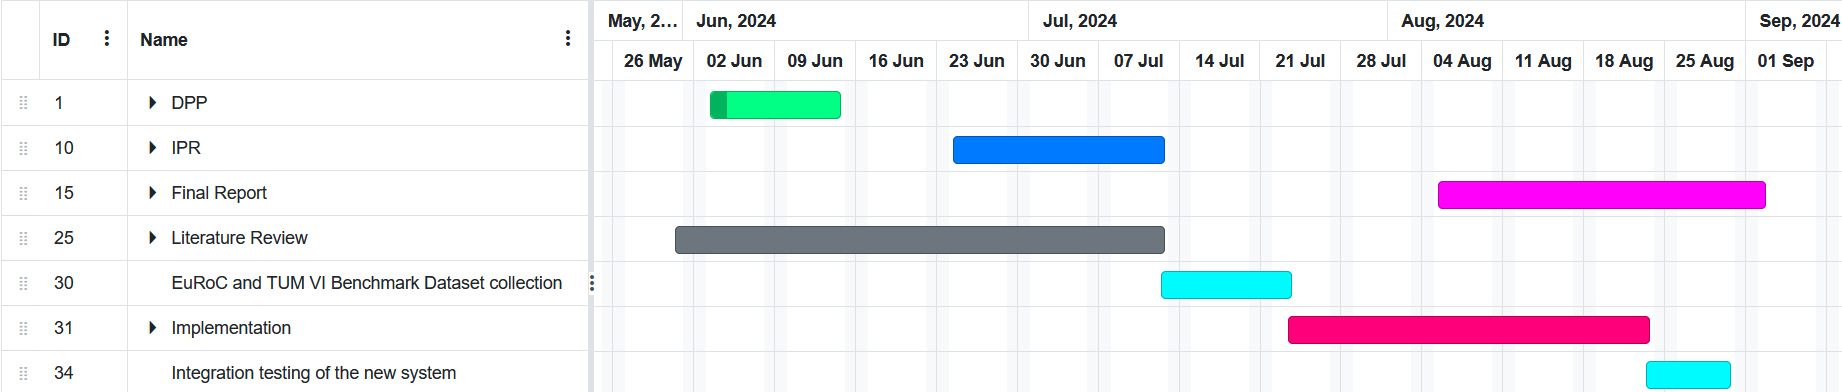
\includegraphics[width=\textwidth,height=\textheight,keepaspectratio]{Images/project plan gantt.png}
        \caption{Gantt chat of project plan}
        \label{fig:Gantt chat of project plan}
    \end{figure}
    \begin{enumerate}
        \item Literature Review	(31-05-2024:12-07-2024)
        \begin{enumerate}
            \item Understanding SLAM and Monocular SLAM	(31-05-2024:04-06-2024)
            \item Understanding ORB SLAM 1,2,3	(04-06-2024:06-06-2024)
            \item Understanding SP SLAM, DX SLAM (06-06-2024:14-06-2024)
            \item Understand ORB SLAM 3 code base (14-06-2024:02-07-2024)
            \item Understand HF-Net	(03-07-2024:12-07-2024)
        \end{enumerate}
        \item EuRoC and TUM VI Benchmark Dataset collection	(12-07-2024:23-07-2024)
        \item Implementation (23-07-2024:23-08-2024)
        \begin{enumerate}
            \item Serialising the HF-Net (23-07-2024:31-07-2024)
            \item writing the wrapper for serialised model in C++ (31-07-2024:08-08-2024)
            \item Unit Testing HF-Net (09-08-2024:12-08-2024)
            \item Intergrate the Model with ORB slam 3 (12-08-2024:23-08-2024)
        \end{enumerate}
        \item Integration testing of the new system	(23-08-2024:26-08-2024)
        \item Validation of the new system with benchmark datasets (26-08-2024:30-08-2024)
    \end{enumerate}
    Milestones:
    \begin{itemize}
        \item Serialising the HF-Net
        \item Integrating HF-Net to ORB-SLAM3
        \item Validation of the new system with benchmark datasets
    \end{itemize}
\end{spacing}

% References
\singlespacing
\printbibliography
\end{document}
